\chapterimage{Pictures/chap05/measure-one180-1260x630.png}
\chapter{颜色和辐射学}\label{chap:颜色和辐射学}
\setcounter{sidenote}{1}

为了精确描述光是怎样被表示和采样以计算图像的,
我们必须首先建立一些\keyindex{辐射学}{radiometry}{}的背景——
\keyindex{电磁辐射}{electromagnetic radiation}{}在环境中的传播研究。
渲染中尤其感兴趣的是\keyindex{波长}{wavelength}{}($\lambda$)大约在
380nm到780nm的电磁辐射\sidenote{译者注:nm即长度单位纳米。$1$纳米=$10^{-9}$米。},
主要是人眼可见光\footnote{可感知波长的完整范围稍微超出了该区间,
但眼睛在这些波长上的敏感性低了许多量级。当绘制光谱曲线时常把范围360-830nm用作保守边界。}。
较短波长($\lambda\approx400\text{nm}$)是偏蓝色的,
中间波长($\lambda\approx550\text{nm}$)是绿色的,
而较长波长($\lambda\approx650\text{nm}$)是红色的。

本章中,我们将介绍描述电磁辐射的四个关键量:
\keyindex{通量}{flux}{}、\keyindex{强度}{intensity}{}、
\keyindex{辐照度}{irradiance}{}和\keyindex{辐亮度}{radiance}{}。
这些辐射量每一个都由它们的\keyindex{光谱功率分布}{spectral power distribution}{}(SPD)——
描述在各波长上光量的关于波长的函数。
pbrt中用定义于\refsec{光谱表示}的类\refvar{Spectrum}{}来表示SPD。

\section{光谱表示}\label{sec:光谱表示}

真实世界物体的SPD可能极其复杂;
\reffig{5.1}展示了荧光灯发光的频谱分布和柠檬皮反射率的频谱分布图。
用SPD做计算的渲染器需要紧实、高效且准确的方式表示像这样的函数。
实践中,可能需要在这些特性间作取舍。
\begin{figure}[htbp]
    \centering
    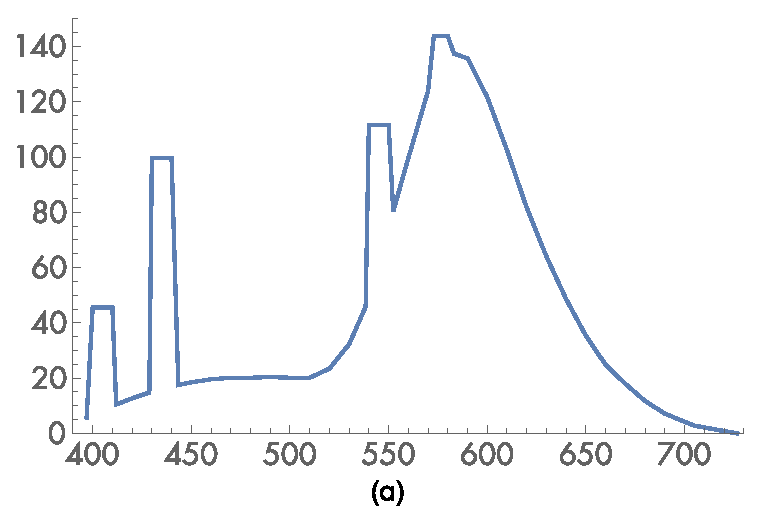
\includegraphics[width=0.45\linewidth]{chap05/fluorescent-spd.eps}\,\nolinebreak
    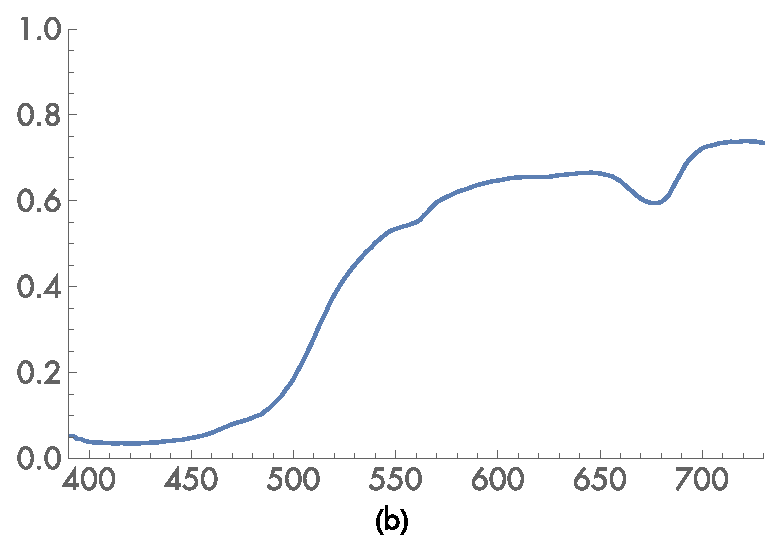
\includegraphics[width=0.45\linewidth]{chap05/lemonskin-spd.eps}
    \caption{(a)荧光灯的频谱分布和(b)柠檬皮的反射率。
    波长400nm左右是偏蓝光,而波长中段是绿色和黄色,波长700nm左右是红光。
    荧光灯的SPD甚至比这里展示的更加尖锐,SPD可归入到10nm范围内;
    它实际上是在单个离散频率上发出大量光。}
    \label{fig:5.1}
\end{figure}

研究这些问题的一般框架可以基于寻找
优良\keyindex{基函数}{basis function}{}以表示SPD的问题来开发。
基函数背后的思想是将可能的SPD函数的无限维空间映射到系数$c_i\in\mathbb{R}$的低维空间。
例如,一个平凡的基函数是常函数$B(\lambda)=1$。
任意SPD可以用等于其平均值的单个系数$c$以该基表示,
这样其近似就为$cB(\lambda)=c$。
很明显这是个很差的近似,因为大多数SPD都比这单个基函数所能准确表示的复杂得多。

在计算机图形学中已经为光谱表示研究了许多不同的基函数;
“扩展阅读”一节引用了关于该话题的许多文献和更多资源。
不同基函数集在关键运算上能提供截然不同的取舍,例如
将任意SPD转换为系数集(将其投影到基上)、
为由基表示的两个SPD之积给定的SPD计算系数等。
本章中,我们将介绍pbrt中可用于光谱的两种表示:\refvar{RGBSpectrum}{},
它遵循经典计算机图形学实践中用表示红、绿和蓝色混合的系数来表示SPD的做法,
以及\refvar{SampledSpectrum}{},它将SPD表示为在一个波长范围上采样点集。

\subsection{光谱类型}\label{sub:光谱类型}
整个pbrt中,我们都根据\refvar{Spectrum}{}类型
用一组特定内建运算符(加法、乘法等)仔细实现涉及SPD的全部计算。
\refvar{Spectrum}{}类型隐藏了所用特定光谱表示的细节,
这样改变系统的这些细节只需要改变\refvar{Spectrum}{}的实现;其他代码可保存不变。
\refvar{Spectrum}{}类型的实现在文件\href{https://github.com/mmp/pbrt-v3/blob/master/src/core/spectrum.h}{\ttfamily core/spectrum.h}和
\href{https://github.com/mmp/pbrt-v3/blob/master/src/core/spectrum.cpp}{\ttfamily core/spectrum.cpp}中。

pbrt中为\refvar{Spectrum}{}类型选择使用哪种光谱表示
在文件\href{https://github.com/mmp/pbrt-v3/blob/master/src/core/pbrt.h}{\ttfamily core/pbrt.h}中
由{\ttfamily typedef}完成。
pbrt默认使用更高效但不太精确的RGB表示。
\begin{lstlisting}
`\initcode{Global Forward Declarations}{=}\initnext{GlobalForwardDeclarations}`
typedef `\refvar{RGBSpectrum}{}` `\initvar{Spectrum}{}`;
// typedef \refvar{SampledSpectrum}{} Spectrum;
\end{lstlisting}

我们还没有把系统编写成在运行时解析选用哪个\refvar{Spectrum}{}表示;
为了切换到不同的表示,整个系统必须重新编译。
这一设计的一个优点是许多各种\refvar{Spectrum}{}方法可以实现为
能被编译器内联\sidenote{译者注:原文inlined。}的短函数,而不是弄成
需要通过相对较慢的虚拟方法调用机制唤起的独立运行函数。
内联像这样的常用短函数能给出性能上的巨大提升。
第二个优点是系统中持有\refvar{Spectrum}{}类型实例的结构可以直接保有它们
而不需要在运行时基于所选的光谱表示动态地分配它们。

\subsection{系数光谱实现}\label{sub:系数光谱实现}
本章实现的两种表示都基于排序固定数目的SPD样本。
因此,
\begin{lstlisting}
`\initcode{Spectrum Declarations}{=}\initnext{SpectrumDeclarations}`
template <int `\initvar{nSpectrumSamples}{}`> class `\initvar{CoefficientSpectrum}{}` {
public:
    `\refcode{CoefficientSpectrum Public Methods}{}`
    `\refcode{CoefficientSpectrum Public Data}{}`
protected:
    `\refcode{CoefficientSpectrum Protected Data}{}`
};
\end{lstlisting}

\begin{lstlisting}
`\initcode{CoefficientSpectrum Public Methods}{=}\initnext{CoefficientSpectrumPublicMethods}`
`\refvar{CoefficientSpectrum}{}`(`\refvar{Float}{}` v = 0.f) {
    for (int i = 0; i < `\refvar{nSpectrumSamples}{}`; ++i)
        `\refvar[CoefficientSpectrum::c]{c}{}`[i] = v;
}
\end{lstlisting}

\begin{lstlisting}
`\initcode{CoefficientSpectrum Protected Data}{=}`
`\refvar{Float}{}` `\initvar[CoefficientSpectrum::c]{c}{}`[`\refvar{nSpectrumSamples}{}`];
\end{lstlisting}

\begin{lstlisting}
`\refcode{CoefficientSpectrum Public Methods}{+=}\lastnext{CoefficientSpectrumPublicMethods}`
bool `\initvar{IsBlack}{}`() const {
    for (int i = 0; i < `\refvar{nSpectrumSamples}{}`; ++i)
        if (`\refvar[CoefficientSpectrum::c]{c}{}`[i] != 0.) return false;
    return true;
}
\end{lstlisting}

{\noindent\hfil$=========$\hfil{\color{red}{施工分割线}}\hfil$=========$\
\section{辐射度学}\label{sec:辐射度学}
 
\keyindex{辐射度学}{radiometry}{}提供了一系列描述光传播与反射的思想和数学工具。
它为贯穿本书剩余部分的渲染算法构建了推导的基础。
有趣的是,辐射度学不是用物理光学基本原理推导产生的,
而是基于穿过空间的粒子流来对光进行抽象并建立的。
因此,尽管辐射度学和\keyindex{麦克斯韦方程组}{Maxwell's equations}{}之间
已经建立了联系,为辐射度学提供了坚实的物理基础,
但像光的\keyindex{偏振}{polarization}{}
\sidenote{译者注:指横波能够朝着不同方向振荡的性质。}
那样的效应并不符合该框架。

\keyindex{辐射转移}{radiative transfer}{}是关于辐射能量转移现象的研究。
它基于辐射度量原则并在\keyindex{几何光学}{geometrical optics}{}
\sidenote{译者注:原文写作geometric optics。}层面上操作,
其中光的宏观性质足以描述光如何与比其波长大得多的物体相交。
与光的\keyindex{波动光学}{wave optics}{}模型中的现象结合并不罕见,
但这些结果需要用辐射转移的基本抽象语言来表达。
(\citet{PREISENDORFER19653}已经将辐射转移理论与
麦克斯韦描述电磁场的经典方程组联系起来。
他的框架既论证了它们的等价性又使得把一个世界观的结果应用到另一个世界观更容易了。
\citet{Fante:81}在该领域做了更多最近的工作。)

用这种方法就能描述光和与其波长大小接近的物体相交,
进而对\keyindex{色散}{dispersion}{}\sidenote{译者注:经典的棱镜色散实验。}
\begin{marginfigure}
    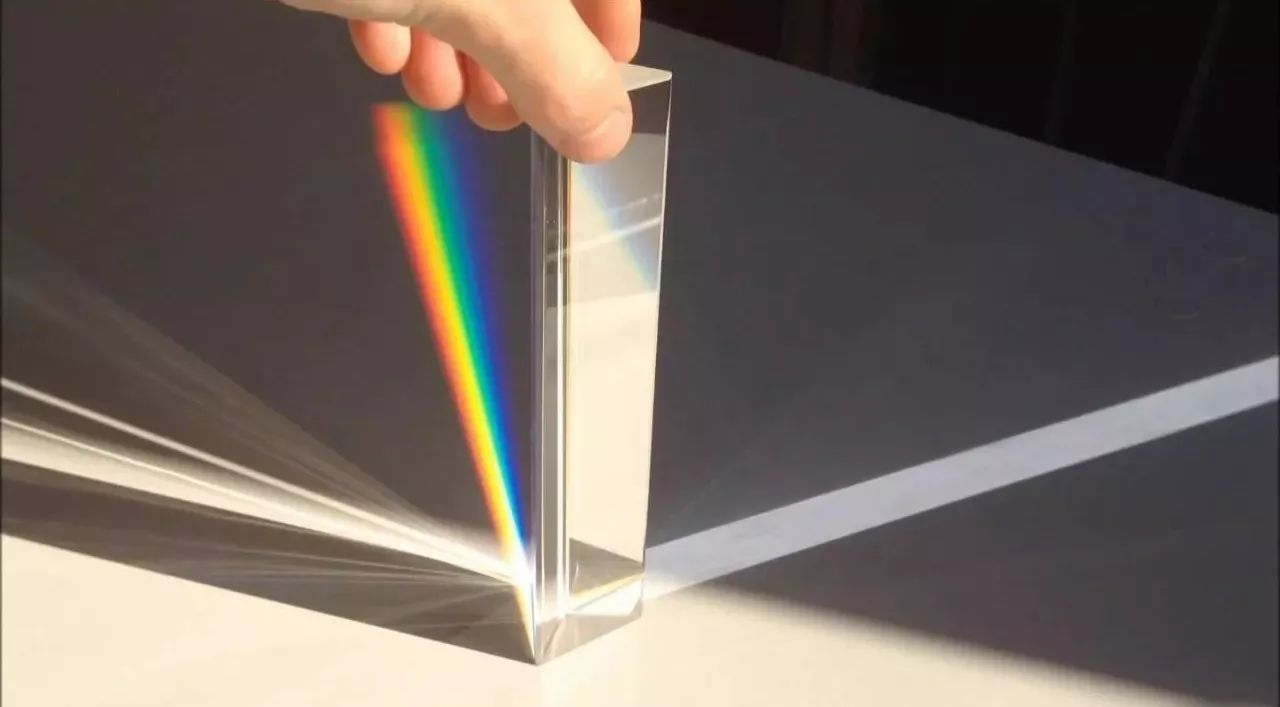
\includegraphics[width=\linewidth]{chap05/dispersion.jpg}
\end{marginfigure}
和\keyindex{干涉}{interference}{}\sidenote{译者注:经典的双缝干涉实验。}
\begin{marginfigure}
    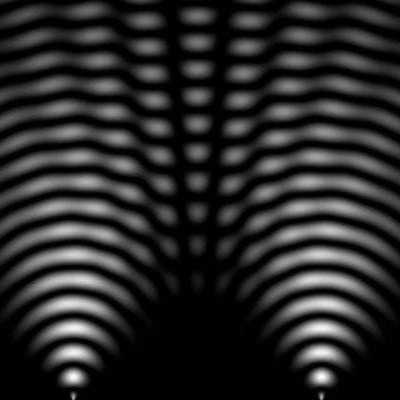
\includegraphics[width=\linewidth]{chap05/interference.jpg}
\end{marginfigure}
等效应建模。
在更精细的细节层面上,需要\keyindex{量子力学}{quantum mechanics}{}来描述光与原子的交互。
幸运的是,解决计算机图形学中的渲染问题不用直接模拟量子力学原理,
故避免了此类方法的复杂性。

在pbrt中,我们将假设几何光学是足够用来描述光与光散射的模型。
这导出了一些整个系统中隐含使用的关于光的行为的基本假设:
\begin{itemize}
    \item \keyindex{线性关系}{linearity}{}:光学系统两个输入的共同效应总是等于每个输入各自效应之和。
    \item \keyindex{能量守恒}{conservation of energy}{}\sidenote{译者注:原文写作energy conservation。}:
    当光从表面或介质散射时,触发的散射不会比它开始时产生更多的能量。
    \item {\sffamily 无偏振}:我们将忽略电磁场的偏振;
    因此,光的唯一相关属性是它关于波长(或等价地,\keyindex{频率}{frequency}{})的分布。
    \item {\sffamily 无}\keyindex{荧光}{fluorescence}{}或\keyindex{磷光}{phosphorescence}{}:
    某一波长的光的行为完全独立于其他波长或时间的光的行为。
    像偏振那样,要包含这些效应并不难,但它们为系统增加的实用价值相对较低。
    \item \keyindex{稳态}{steady state}{}:假设环境中的光达到平衡,
    所以其辐射分布不随时间变化。在现实场景中这对于光几乎是一瞬间发生的,
    所以在实践中这没什么限制。注意磷光也违反了稳态假设。
\end{itemize}

采用几何光学模型最明显的损失是很难考虑\keyindex{衍射}{diffraction}{}和干涉效应。
如\citet[p. 24]{PREISENDORFER19653}所述,这是个很难解决的问题,
例如,当存在这些效应时两区域的总通量不一定等于每个区域各自接收的功率之和。

\subsection{基本量}\label{sub:基本量}
有四个辐射度量数量\sidenote{译者注:依据中国国家标准GB 3102.6-93,
这些量的名称大都可以省略“射”字,例如“辐射出射度”也可以称作
“辐射出度”“辐出射度”“辐出度”,以此类推。后续译文将视情况使用全称或简称。}
是渲染的核心:\keyindex{通量}{flux}{}、
\keyindex{辐射照度}{irradiance}{}/\keyindex{辐射出射度}{radiant exitance}{}、
\keyindex{强度}{intensity}{}和\keyindex{辐射亮度}{radiance}{}。
它们每个都可以从能量(单位为焦耳)依次对时间、面积和方向取极限推导出来。
所有这些辐射度量数量一般都依赖于波长。
对于本章的剩余部分,我们不再明确这一依赖关系,但记住这一性质是很重要的。

\subsubsection*{能量}
我们的起点是\keyindex{能量}{energy}{}
\sidenote{译者注:也称为\keyindex{辐射能}{radiant energy}{}。},
单位为\keyindex{焦耳}{joule}{}(焦,J)
\sidenote{译者注:{\normalfont $1\text{J}=1\text{kg}\cdot\text{m}^2/\text{s}^2$。}}。
照射源发射\keyindex{光子}{photon}{},
每个光子有特定波长并携带特定数量的能量。
所有这些基本辐射度量数量实际都是对光子的不同度量。
波长为$\lambda$的一个光子携带能量为
\begin{align*}
    Q=\frac{hc}{\lambda}\, ,
\end{align*}
其中$c$是光的速率
\sidenote{译者注:指真空环境下的光速;
原文写作{\normalfont $299,472,458\text{m}/\text{s}$},此处更正为国际标准值。}
即$299,792,458\text{m}/\text{s}$,$h$为\keyindex{普朗克常数}{Planck constant}{}
\sidenote{译者注:其单位可化简为{\normalfont$\text{J}\cdot\text{s}$}。},
$h\approx6.626\times10^{-34}\text{kg}\cdot\text{m}^2/\text{s}$。

\subsubsection*{通量}
能量度量了一段时间上的\keyindex{功}{work}{},
尽管渲染一般使用稳态假设,但我们最感兴趣的是度量一瞬间的光。
\keyindex{辐射能通量}{radiant energy flux}{}
\sidenote{译者注:也称辐射通量、辐通量;原文写作radiant flux。},
也称为\keyindex{辐射功率}{radiant power}{}\sidenote{译者注:原文写作power。},
是单位时间内穿过表面或空间区域的能量总量。
辐射通量可以通过求每个微分时间内微分能量的极限算出:
\begin{align*}
    \varPhi=\lim\limits_{\Delta t\rightarrow 0}{\frac{\Delta Q}{\Delta t}}=\frac{\mathrm{d}Q}{\mathrm{d}t}\, .
\end{align*}
它的单位是焦耳$/$秒,即更常见的\keyindex{瓦特}{watt}{}(瓦,W)。

例如,设一光源在一小时内发射了$Q=200,000\text{J}$,
如果这一小时内任何时候发射的能量都相同,
我们可以求得该光源的通量为
\begin{align*}
    \varPhi=200,000\text{J}/3600\text{s}\approx 55.6\text{W}\, .
\end{align*}

反之,设通量是时间的函数,我们可以在一段时间上积分算出总能量:
\begin{align*}
    Q=\int_{t_0}^{t_1}\varPhi(t)\mathrm{d}t\, .
\end{align*}

注意这里我们的记号有些不正式:在其他问题中,因为光子实际上是离散量子,
对趋近于零的微分时间取极限没有实际意义。
但对于渲染目的,光子数量相比于我们感兴趣的度量是巨大的,在实践中这一细节不会有问题。

来自光源的总辐射一般用通量描述。
\reffig{5.6}展示了来自一个点光源的通量由
穿过包围该光源的假想球面的能量总量度量。
注意\reffig{5.6}中在两个球面的任意一个上度量的通量总量是一样的——
尽管穿过大球任意局部的能量比小球少,
但大球的面积更大,意味着总通量一样多。
\begin{figure}[htbp]
    \centering%LaTeX with PSTricks extensions
%%Creator: Inkscape 1.0.1 (3bc2e813f5, 2020-09-07)
%%Please note this file requires PSTricks extensions
\psset{xunit=.5pt,yunit=.5pt,runit=.5pt}
\begin{pspicture}(254.8999939,254.8999939)
{
\newrgbcolor{curcolor}{0 0 0}
\pscustom[linewidth=1,linecolor=curcolor]
{
\newpath
\moveto(188.40000153,127.20999146)
\curveto(188.40000153,151.66779751)(173.6668771,173.71750129)(151.07121577,183.07656872)
\curveto(128.47560051,192.43561706)(102.46763049,187.26077332)(85.17342447,169.96656729)
\curveto(67.87921844,152.67236127)(62.7043747,126.66439125)(72.06342304,104.06877599)
\curveto(81.42249047,81.47311466)(103.47219425,66.73999023)(127.93000031,66.73999023)
\curveto(152.38780636,66.73999023)(174.43751014,81.47311466)(183.79657757,104.06877599)
\curveto(193.15562591,126.66439125)(187.98078217,152.67236127)(170.68657615,169.96656729)
\curveto(153.39237012,187.26077332)(127.3844001,192.43561706)(104.78878484,183.07656872)
\curveto(82.19312351,173.71750129)(67.45999908,151.66779751)(67.45999908,127.20999146)
\curveto(67.45999908,102.7521854)(82.19312351,80.70248162)(104.78878484,71.34341419)
\curveto(127.3844001,61.98436585)(153.39237012,67.15920959)(170.68657615,84.45341562)
\curveto(187.98078217,101.74762164)(193.15562591,127.75559166)(183.79657757,150.35120692)
\curveto(174.43751014,172.94686825)(152.38780636,187.67999268)(127.93000031,187.67999268)
\curveto(103.47219425,187.67999268)(81.42249047,172.94686825)(72.06342304,150.35120692)
\curveto(62.7043747,127.75559166)(67.87921844,101.74762164)(85.17342447,84.45341562)
\curveto(102.46763049,67.15920959)(128.47560051,61.98436585)(151.07121577,71.34341419)
\curveto(173.6668771,80.70248162)(188.40000153,102.7521854)(188.40000153,127.20999146)
\closepath
}
}
{
\newrgbcolor{curcolor}{0 0 0}
\pscustom[linewidth=1,linecolor=curcolor]
{
\newpath
\moveto(254.3999939,127.44999695)
\curveto(254.3999939,178.7964223)(223.46944879,225.08730657)(176.03238777,244.73562073)
\curveto(128.59542349,264.38389481)(73.99460246,253.5198898)(37.68735328,217.21264062)
\curveto(1.3801041,180.90539144)(-9.48390091,126.30457041)(10.16437317,78.86760613)
\curveto(29.81268733,31.43054511)(76.1035716,0.5)(127.44999695,0.5)
\curveto(178.7964223,0.5)(225.08730657,31.43054511)(244.73562073,78.86760613)
\curveto(264.38389481,126.30457041)(253.5198898,180.90539144)(217.21264062,217.21264062)
\curveto(180.90539144,253.5198898)(126.30457041,264.38389481)(78.86760613,244.73562073)
\curveto(31.43054511,225.08730657)(0.5,178.7964223)(0.5,127.44999695)
\curveto(0.5,76.1035716)(31.43054511,29.81268733)(78.86760613,10.16437317)
\curveto(126.30457041,-9.48390091)(180.90539144,1.3801041)(217.21264062,37.68735328)
\curveto(253.5198898,73.99460246)(264.38389481,128.59542349)(244.73562073,176.03238777)
\curveto(225.08730657,223.46944879)(178.7964223,254.3999939)(127.44999695,254.3999939)
\curveto(76.1035716,254.3999939)(29.81268733,223.46944879)(10.16437317,176.03238777)
\curveto(-9.48390091,128.59542349)(1.3801041,73.99460246)(37.68735328,37.68735328)
\curveto(73.99460246,1.3801041)(128.59542349,-9.48390091)(176.03238777,10.16437317)
\curveto(223.46944879,29.81268733)(254.3999939,76.1035716)(254.3999939,127.44999695)
\closepath
}
}
{
\newrgbcolor{curcolor}{0.98823529 0.93333334 0.12941177}
\pscustom[linestyle=none,fillstyle=solid,fillcolor=curcolor]
{
\newpath
\moveto(132.21,146.9699939)
\lineto(130.63,137.2899939)
\lineto(135.58,145.7499939)
\lineto(132.25,136.5299939)
\lineto(138.67,143.9399939)
\lineto(133.71,135.4899939)
\lineto(141.38,141.5799939)
\lineto(134.95,134.1899939)
\lineto(143.61,138.7699939)
\lineto(135.93,132.6899939)
\lineto(145.29,135.5999939)
\lineto(136.62,131.0299939)
\lineto(146.35,132.1799939)
\lineto(136.99,129.2799939)
\lineto(146.77,128.6099939)
\lineto(137.03,127.4799939)
\lineto(146.52,125.0399939)
\lineto(136.74,125.7099939)
\lineto(145.62,121.5599939)
\lineto(136.14,124.0299939)
\lineto(144.1,118.3099939)
\lineto(135.23,122.4799939)
\lineto(142.01,115.3999939)
\lineto(134.05,121.1299939)
\lineto(139.42,112.9199939)
\lineto(132.65,120.0099939)
\lineto(136.41,110.9599939)
\lineto(131.06,119.1699939)
\lineto(133.1,109.5899939)
\lineto(129.35,118.6399939)
\lineto(129.59,108.8399939)
\lineto(127.57,118.4299939)
\lineto(126,108.7599939)
\lineto(125.78,118.5599939)
\lineto(122.47,109.3299939)
\lineto(124.04,118.9999939)
\lineto(119.09,110.5499939)
\lineto(122.42,119.7699939)
\lineto(116,112.3599939)
\lineto(120.96,120.8099939)
\lineto(113.29,114.7099939)
\lineto(119.72,122.1099939)
\lineto(111.06,117.5199939)
\lineto(118.74,123.6099939)
\lineto(109.38,120.6999939)
\lineto(118.05,125.2699939)
\lineto(108.32,124.1199939)
\lineto(117.68,127.0199939)
\lineto(107.9,127.6799939)
\lineto(117.64,128.8099939)
\lineto(108.15,131.2599939)
\lineto(117.93,130.5799939)
\lineto(109.05,134.7299939)
\lineto(118.53,132.2699939)
\lineto(110.57,137.9799939)
\lineto(119.44,133.8199939)
\lineto(112.66,140.8999939)
\lineto(120.62,135.1699939)
\lineto(115.25,143.3699939)
\lineto(122.02,136.2899939)
\lineto(118.26,145.3399939)
\lineto(123.61,137.1199939)
\lineto(121.57,146.7099939)
\lineto(125.32,137.6599939)
\lineto(125.08,147.4599939)
\lineto(127.1,137.8699939)
\lineto(128.66,147.5399939)
\lineto(128.89,137.7399939)
\closepath
}
}
{
\newrgbcolor{curcolor}{0 0 0}
\pscustom[linewidth=0.30000001,linecolor=curcolor]
{
\newpath
\moveto(132.21,146.9699939)
\lineto(130.63,137.2899939)
\lineto(135.58,145.7499939)
\lineto(132.25,136.5299939)
\lineto(138.67,143.9399939)
\lineto(133.71,135.4899939)
\lineto(141.38,141.5799939)
\lineto(134.95,134.1899939)
\lineto(143.61,138.7699939)
\lineto(135.93,132.6899939)
\lineto(145.29,135.5999939)
\lineto(136.62,131.0299939)
\lineto(146.35,132.1799939)
\lineto(136.99,129.2799939)
\lineto(146.77,128.6099939)
\lineto(137.03,127.4799939)
\lineto(146.52,125.0399939)
\lineto(136.74,125.7099939)
\lineto(145.62,121.5599939)
\lineto(136.14,124.0299939)
\lineto(144.1,118.3099939)
\lineto(135.23,122.4799939)
\lineto(142.01,115.3999939)
\lineto(134.05,121.1299939)
\lineto(139.42,112.9199939)
\lineto(132.65,120.0099939)
\lineto(136.41,110.9599939)
\lineto(131.06,119.1699939)
\lineto(133.1,109.5899939)
\lineto(129.35,118.6399939)
\lineto(129.59,108.8399939)
\lineto(127.57,118.4299939)
\lineto(126,108.7599939)
\lineto(125.78,118.5599939)
\lineto(122.47,109.3299939)
\lineto(124.04,118.9999939)
\lineto(119.09,110.5499939)
\lineto(122.42,119.7699939)
\lineto(116,112.3599939)
\lineto(120.96,120.8099939)
\lineto(113.29,114.7099939)
\lineto(119.72,122.1099939)
\lineto(111.06,117.5199939)
\lineto(118.74,123.6099939)
\lineto(109.38,120.6999939)
\lineto(118.05,125.2699939)
\lineto(108.32,124.1199939)
\lineto(117.68,127.0199939)
\lineto(107.9,127.6799939)
\lineto(117.64,128.8099939)
\lineto(108.15,131.2599939)
\lineto(117.93,130.5799939)
\lineto(109.05,134.7299939)
\lineto(118.53,132.2699939)
\lineto(110.57,137.9799939)
\lineto(119.44,133.8199939)
\lineto(112.66,140.8999939)
\lineto(120.62,135.1699939)
\lineto(115.25,143.3699939)
\lineto(122.02,136.2899939)
\lineto(118.26,145.3399939)
\lineto(123.61,137.1199939)
\lineto(121.57,146.7099939)
\lineto(125.32,137.6599939)
\lineto(125.08,147.4599939)
\lineto(127.1,137.8699939)
\lineto(128.66,147.5399939)
\lineto(128.89,137.7399939)
\closepath
}
}
{
\newrgbcolor{curcolor}{0 0 0}
\pscustom[linewidth=1,linecolor=curcolor]
{
\newpath
\moveto(127.12999725,173.73999023)
\lineto(127.12999725,153.51999664)
}
}
{
\newrgbcolor{curcolor}{0 0 0}
\pscustom[linestyle=none,fillstyle=solid,fillcolor=curcolor]
{
\newpath
\moveto(121.63,168.8399939)
\lineto(127.13,173.0899939)
\lineto(132.63,168.8399939)
\lineto(127.13,181.8499939)
\closepath
}
}
{
\newrgbcolor{curcolor}{0.65098041 0.65098041 0.65098041}
\pscustom[linestyle=none,fillstyle=solid,fillcolor=curcolor]
{
\newpath
\moveto(122.83,170.3899939)
\lineto(127.13,180.5399939)
\lineto(127.13,173.7299939)
\closepath
}
}
{
\newrgbcolor{curcolor}{0.40000001 0.40000001 0.40000001}
\pscustom[linestyle=none,fillstyle=solid,fillcolor=curcolor]
{
\newpath
\moveto(131.43,170.3899939)
\lineto(127.13,180.5399939)
\lineto(127.13,173.7299939)
\closepath
}
}
{
\newrgbcolor{curcolor}{0 0 0}
\pscustom[linewidth=1,linecolor=curcolor]
{
\newpath
\moveto(127.12999725,233.55999374)
\lineto(127.12999725,198.08999252)
}
}
{
\newrgbcolor{curcolor}{0 0 0}
\pscustom[linestyle=none,fillstyle=solid,fillcolor=curcolor]
{
\newpath
\moveto(121.63,228.6499939)
\lineto(127.13,232.9099939)
\lineto(132.63,228.6499939)
\lineto(127.13,241.6699939)
\closepath
}
}
{
\newrgbcolor{curcolor}{0.65098041 0.65098041 0.65098041}
\pscustom[linestyle=none,fillstyle=solid,fillcolor=curcolor]
{
\newpath
\moveto(122.83,230.2099939)
\lineto(127.13,240.3499939)
\lineto(127.13,233.5399939)
\closepath
}
}
{
\newrgbcolor{curcolor}{0.40000001 0.40000001 0.40000001}
\pscustom[linestyle=none,fillstyle=solid,fillcolor=curcolor]
{
\newpath
\moveto(131.43,230.2099939)
\lineto(127.13,240.3499939)
\lineto(127.13,233.5399939)
\closepath
}
}
{
\newrgbcolor{curcolor}{0 0 0}
\pscustom[linewidth=1,linecolor=curcolor]
{
\newpath
\moveto(107.52999878,169.63999176)
\lineto(116.30000305,151.42999268)
}
}
{
\newrgbcolor{curcolor}{0 0 0}
\pscustom[linestyle=none,fillstyle=solid,fillcolor=curcolor]
{
\newpath
\moveto(104.7,162.8299939)
\lineto(107.81,169.0599939)
\lineto(114.62,167.6099939)
\lineto(104.01,176.9499939)
\closepath
}
}
{
\newrgbcolor{curcolor}{0.65098041 0.65098041 0.65098041}
\pscustom[linestyle=none,fillstyle=solid,fillcolor=curcolor]
{
\newpath
\moveto(105.11,164.7599939)
\lineto(104.58,175.7599939)
\lineto(107.54,169.6299939)
\closepath
}
}
{
\newrgbcolor{curcolor}{0.40000001 0.40000001 0.40000001}
\pscustom[linestyle=none,fillstyle=solid,fillcolor=curcolor]
{
\newpath
\moveto(112.85,168.4899939)
\lineto(104.58,175.7599939)
\lineto(107.54,169.6299939)
\closepath
}
}
{
\newrgbcolor{curcolor}{0 0 0}
\pscustom[linewidth=1,linecolor=curcolor]
{
\newpath
\moveto(81.55999756,223.53999329)
\lineto(96.95999908,191.5799942)
}
}
{
\newrgbcolor{curcolor}{0 0 0}
\pscustom[linestyle=none,fillstyle=solid,fillcolor=curcolor]
{
\newpath
\moveto(78.74,216.7199939)
\lineto(81.85,222.9499939)
\lineto(88.65,221.4999939)
\lineto(78.05,230.8299939)
\closepath
}
}
{
\newrgbcolor{curcolor}{0.65098041 0.65098041 0.65098041}
\pscustom[linestyle=none,fillstyle=solid,fillcolor=curcolor]
{
\newpath
\moveto(79.14,218.6499939)
\lineto(78.62,229.6499939)
\lineto(81.57,223.5199939)
\closepath
}
}
{
\newrgbcolor{curcolor}{0.40000001 0.40000001 0.40000001}
\pscustom[linestyle=none,fillstyle=solid,fillcolor=curcolor]
{
\newpath
\moveto(86.89,222.3799939)
\lineto(78.62,229.6499939)
\lineto(81.57,223.5199939)
\closepath
}
}
{
\newrgbcolor{curcolor}{0 0 0}
\pscustom[linewidth=1,linecolor=curcolor]
{
\newpath
\moveto(92.12999725,156.56999207)
\lineto(107.69999695,143.66999054)
}
}
{
\newrgbcolor{curcolor}{0 0 0}
\pscustom[linestyle=none,fillstyle=solid,fillcolor=curcolor]
{
\newpath
\moveto(92.4,149.1999939)
\lineto(92.63,156.1599939)
\lineto(99.42,157.6799939)
\lineto(85.89,161.7399939)
\closepath
}
}
{
\newrgbcolor{curcolor}{0.65098041 0.65098041 0.65098041}
\pscustom[linestyle=none,fillstyle=solid,fillcolor=curcolor]
{
\newpath
\moveto(91.97,151.1199939)
\lineto(86.9,160.9099939)
\lineto(92.15,156.5599939)
\closepath
}
}
{
\newrgbcolor{curcolor}{0.40000001 0.40000001 0.40000001}
\pscustom[linestyle=none,fillstyle=solid,fillcolor=curcolor]
{
\newpath
\moveto(97.45,157.7399939)
\lineto(86.9,160.9099939)
\lineto(92.15,156.5599939)
\closepath
}
}
{
\newrgbcolor{curcolor}{0 0 0}
\pscustom[linewidth=1,linecolor=curcolor]
{
\newpath
\moveto(46.06999969,194.73999405)
\lineto(73.38999939,172.10999298)
}
}
{
\newrgbcolor{curcolor}{0 0 0}
\pscustom[linestyle=none,fillstyle=solid,fillcolor=curcolor]
{
\newpath
\moveto(46.34,187.3699939)
\lineto(46.57,194.3299939)
\lineto(53.37,195.8499939)
\lineto(39.83,199.9199939)
\closepath
}
}
{
\newrgbcolor{curcolor}{0.65098041 0.65098041 0.65098041}
\pscustom[linestyle=none,fillstyle=solid,fillcolor=curcolor]
{
\newpath
\moveto(45.91,189.2899939)
\lineto(40.84,199.0799939)
\lineto(46.09,194.7299939)
\closepath
}
}
{
\newrgbcolor{curcolor}{0.40000001 0.40000001 0.40000001}
\pscustom[linestyle=none,fillstyle=solid,fillcolor=curcolor]
{
\newpath
\moveto(51.4,195.9099939)
\lineto(40.84,199.0799939)
\lineto(46.09,194.7299939)
\closepath
}
}
{
\newrgbcolor{curcolor}{0 0 0}
\pscustom[linewidth=1,linecolor=curcolor]
{
\newpath
\moveto(147.63000488,169.3299942)
\lineto(138.8500061,151.11999512)
}
}
{
\newrgbcolor{curcolor}{0 0 0}
\pscustom[linestyle=none,fillstyle=solid,fillcolor=curcolor]
{
\newpath
\moveto(140.54,167.2999939)
\lineto(147.34,168.7499939)
\lineto(150.45,162.5199939)
\lineto(151.14,176.6299939)
\closepath
}
}
{
\newrgbcolor{curcolor}{0.65098041 0.65098041 0.65098041}
\pscustom[linestyle=none,fillstyle=solid,fillcolor=curcolor]
{
\newpath
\moveto(142.3,168.1799939)
\lineto(150.57,175.4499939)
\lineto(147.62,169.3199939)
\closepath
}
}
{
\newrgbcolor{curcolor}{0.40000001 0.40000001 0.40000001}
\pscustom[linestyle=none,fillstyle=solid,fillcolor=curcolor]
{
\newpath
\moveto(150.04,164.4499939)
\lineto(150.57,175.4499939)
\lineto(147.62,169.3199939)
\closepath
}
}
{
\newrgbcolor{curcolor}{0 0 0}
\pscustom[linewidth=1,linecolor=curcolor]
{
\newpath
\moveto(173.58999634,223.21999359)
\lineto(158.19000244,191.26999283)
}
}
{
\newrgbcolor{curcolor}{0 0 0}
\pscustom[linestyle=none,fillstyle=solid,fillcolor=curcolor]
{
\newpath
\moveto(166.5,221.1899939)
\lineto(173.31,222.6399939)
\lineto(176.42,216.4099939)
\lineto(177.11,230.5199939)
\closepath
}
}
{
\newrgbcolor{curcolor}{0.65098041 0.65098041 0.65098041}
\pscustom[linestyle=none,fillstyle=solid,fillcolor=curcolor]
{
\newpath
\moveto(168.26,222.0699939)
\lineto(176.54,229.3399939)
\lineto(173.58,223.2099939)
\closepath
}
}
{
\newrgbcolor{curcolor}{0.40000001 0.40000001 0.40000001}
\pscustom[linestyle=none,fillstyle=solid,fillcolor=curcolor]
{
\newpath
\moveto(176.01,218.3399939)
\lineto(176.54,229.3399939)
\lineto(173.58,223.2099939)
\closepath
}
}
{
\newrgbcolor{curcolor}{0 0 0}
\pscustom[linewidth=1,linecolor=curcolor]
{
\newpath
\moveto(163.02000427,156.25999451)
\lineto(147.44999695,143.35999298)
}
}
{
\newrgbcolor{curcolor}{0 0 0}
\pscustom[linestyle=none,fillstyle=solid,fillcolor=curcolor]
{
\newpath
\moveto(155.73,157.3699939)
\lineto(162.52,155.8499939)
\lineto(162.75,148.8899939)
\lineto(169.26,161.4299939)
\closepath
}
}
{
\newrgbcolor{curcolor}{0.65098041 0.65098041 0.65098041}
\pscustom[linestyle=none,fillstyle=solid,fillcolor=curcolor]
{
\newpath
\moveto(157.7,157.4399939)
\lineto(168.25,160.5999939)
\lineto(163.01,156.2499939)
\closepath
}
}
{
\newrgbcolor{curcolor}{0.40000001 0.40000001 0.40000001}
\pscustom[linestyle=none,fillstyle=solid,fillcolor=curcolor]
{
\newpath
\moveto(163.18,150.8199939)
\lineto(168.25,160.5999939)
\lineto(163.01,156.2499939)
\closepath
}
}
{
\newrgbcolor{curcolor}{0 0 0}
\pscustom[linewidth=1,linecolor=curcolor]
{
\newpath
\moveto(209.08000183,194.42999268)
\lineto(181.77000427,171.79999542)
}
}
{
\newrgbcolor{curcolor}{0 0 0}
\pscustom[linestyle=none,fillstyle=solid,fillcolor=curcolor]
{
\newpath
\moveto(201.79,195.5399939)
\lineto(208.58,194.0199939)
\lineto(208.81,187.0599939)
\lineto(215.32,199.5999939)
\closepath
}
}
{
\newrgbcolor{curcolor}{0.65098041 0.65098041 0.65098041}
\pscustom[linestyle=none,fillstyle=solid,fillcolor=curcolor]
{
\newpath
\moveto(203.75,195.6099939)
\lineto(214.31,198.7699939)
\lineto(209.06,194.4199939)
\closepath
}
}
{
\newrgbcolor{curcolor}{0.40000001 0.40000001 0.40000001}
\pscustom[linestyle=none,fillstyle=solid,fillcolor=curcolor]
{
\newpath
\moveto(209.24,188.9799939)
\lineto(214.31,198.7699939)
\lineto(209.06,194.4199939)
\closepath
}
}
\end{pspicture}

    \caption{辐射通量$\varPhi$度量穿过表面或空间区域的能量。
    这里来自一个点光源的通量由包围它的球来度量。}
    \label{fig:5.6}
\end{figure}

\subsubsection*{辐射照度与辐射出射度}

\subsection{亮度和光度学}\label{sub:亮度和光度学}

\section{表面反射}\label{sec:表面反射}

当光入射到表面时,表面会散射该光,将其一部分反射回环境中。
有两个需要描述的效应以对反射建模:反射光的光谱分布和其方向分布。
例如,柠檬皮大都吸收了蓝波长的光而反射了大部分红和绿波长的光
(回想\reffig{5.1}中柠檬皮的反射SPD)。
因此,当用白光照射它时,其颜色是黄色。
无论从哪个方向观察,皮的颜色都相当一致,
但有的方向会有\keyindex{高光}{highlight}{}——会看见与其说黄色不如说白色的更亮区域
\sidenote{译者注:有高光区的柠檬照片。}。
\begin{marginfigure}
    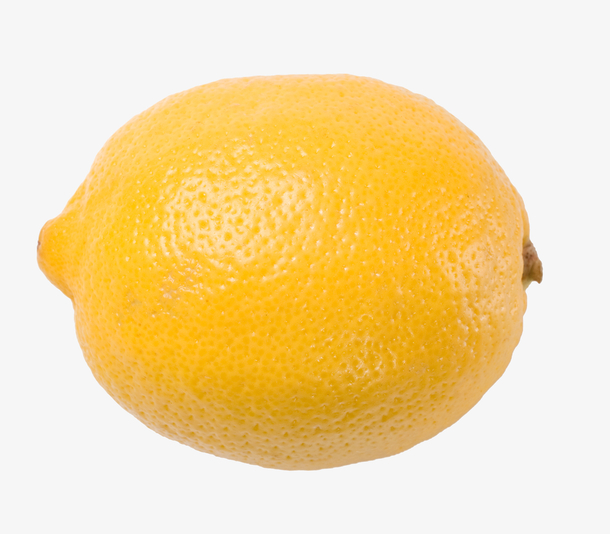
\includegraphics[width=\linewidth]{chap05/lemon.jpg}
\end{marginfigure}
相反,镜子一点反射的光几乎完全取决于观察方向。
在镜子的固定点上,当观察角度变化时,镜子反射的物体也随之变化。

来自\keyindex{半透明}{translucent}{}表面的反射更复杂;
从皮和叶子到蜡和液体的各种材料都
表现出\keyindex{次表面光传输}{subsurface light transport}{light transport光传输},
即进入表面一点的光在有一定距离的地方退出。
(例如考虑在一个人的嘴巴里开手电筒会让他的脸颊被照亮,
因为进入脸颊内侧的光穿过了皮肤并从脸上退出。)

有两种抽象来为光的反射描述这些机制:
\refsub{BRDF}和\refsub{BSSRDF}分别介绍的BRDF和BSSRDF。
BRDF描述一点的表面反射而忽略次表面光传输效应;
对于不受该传输机制明显影响的材料,
这一简化会减少报错并让渲染算法的实现高效得多。
BSSRDF推广了BRDF并描述来自半透明材料光反射的更一般设置。

\subsection{BRDF}\label{sub:BRDF}
\keyindex{双向反射分布函数}{bidirectional reflectance distribution function}{}(BRDF)
为描述来自表面的反射给出了形式。考虑\reffig{5.18}中的设置:
我们想知道,作为沿方向${\bm\omega}_{\mathrm{i}}$
入射辐亮度$L_{\mathrm{i}}({\bm p},{\bm\omega}_{\mathrm{i}})$的结果,
在朝向观察者的方向${\bm\omega}_{\mathrm{o}}$中
有多少辐射亮度$L_{\mathrm{o}}({\bm p},{\bm\omega}_{\mathrm{o}})$离开表面。
\begin{figure}[htbp]
    \centering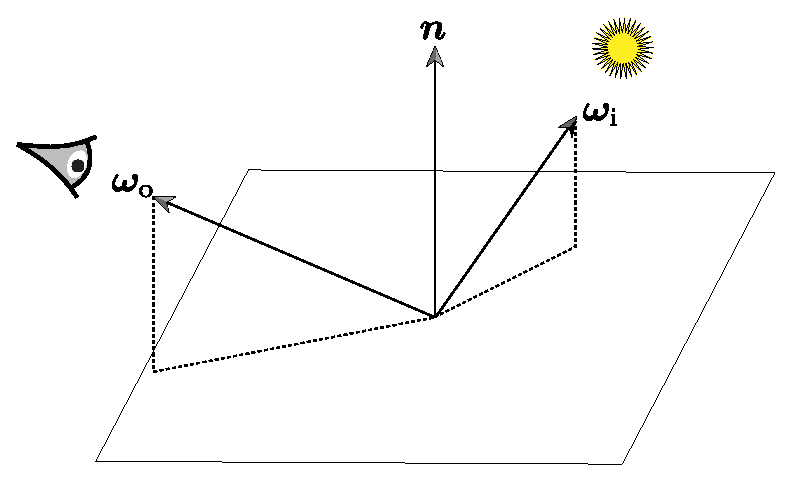
\includegraphics[width=0.5\linewidth]{chap05/BRDF.eps}
    \caption{BRDF。双向反射分布函数是在一对方向${\bm\omega}_{\mathrm{i}}$
        和${\bm\omega}_{\mathrm{o}}$上描述有多少沿${\bm\omega}_{\mathrm{i}}$
        入射的光从表面朝方向${\bm\omega}_{\mathrm{o}}$散射的4D函数。}
    \label{fig:5.18}
\end{figure}

如果方向${\bm\omega}_{\mathrm{i}}$视作方向的微分锥,则$\bm p$处的微分辐照度是
\begin{align}\label{eq:5.7}
    \mathrm{d}E({\bm p},{\bm\omega}_{\mathrm{i}})=L_{\mathrm{i}}({\bm p},{\bm\omega}_{\mathrm{i}})\cos\theta_{\mathrm{i}}\mathrm{d}{\bm\omega}_{\mathrm{i}}\, .
\end{align}

要被反射到方向${\bm\omega}_{\mathrm{o}}$的辐射亮度微分量取决于该辐射照度。
因为几何光学的线性假设,反射的微分辐射亮度正比于辐射照度
\begin{align*}
    \mathrm{d}L_{\mathrm{o}}({\bm p},{\bm\omega}_{\mathrm{o}})\propto\mathrm{d}E({\bm p},{\bm\omega}_{\mathrm{i}})\, .
\end{align*}

比例常数为这对特定方向${\bm\omega}_{\mathrm{i}}$和${\bm\omega}_{\mathrm{o}}$定义了曲面的BRDF:
\begin{align}\label{eq:5.8}
    f_{\mathrm{r}}({\bm p},{\bm \omega}_\mathrm{o},{\bm \omega}_\mathrm{i})=\frac{\mathrm{d}L_{\mathrm{o}}({\bm p},{\bm\omega}_{\mathrm{o}})}{\mathrm{d}E({\bm p},{\bm\omega}_{\mathrm{i}})}=\frac{\mathrm{d}L_{\mathrm{o}}({\bm p},{\bm\omega}_{\mathrm{o}})}{L_{\mathrm{i}}({\bm p},{\bm\omega}_{\mathrm{i}})\cos\theta_{\mathrm{i}}\mathrm{d}{\bm\omega}_{\mathrm{i}}}\, .
\end{align}

基于物理的BRDF有两个重要性质:
\begin{enumerate}
    \item \keyindex{互易性}{reciprocity}{}:对所有方向对${\bm\omega}_{\mathrm{i}}$和${\bm\omega}_{\mathrm{o}}$,
          $f_{\mathrm{r}}({\bm p},{\bm \omega}_\mathrm{i},{\bm \omega}_\mathrm{o})=f_{\mathrm{r}}({\bm p},{\bm \omega}_\mathrm{o},{\bm \omega}_\mathrm{i})$。
    \item {\sffamily 能量守恒}:光反射的总能量少于或等于入射光的能量。
          对于所有方向${\bm\omega}_{\mathrm{o}}$,
          \begin{align*}
              \int\limits_{H^2({\bm n})}f_{\mathrm{r}}({\bm p},{\bm \omega}_\mathrm{o},{\bm \omega}')\cos\theta'\mathrm{d}{\bm\omega}'\le1\, .
          \end{align*}
\end{enumerate}

曲面的\keyindex{双向透射分布函数}{bidirectional transmittance distribution function}{}
(BTDF)描述透射光的分布,可以用和BRDF一样的方法定义。
BTDF一般表示为$f_{\mathrm{t}}({\bm p},{\bm \omega}_\mathrm{o},{\bm \omega}_\mathrm{i})$,
其中${\bm\omega}_{\mathrm{i}}$和${\bm\omega}_{\mathrm{o}}$在绕$\bm p$的相对半球内。
要注意的是,BTDF不遵循上面定义的互异性;
我们将在\refsec{镜面反射与透射}和\refsub{非对称散射}详细讨论该问题。

为了等式的方便,我们把统一考虑时的BRDF和BTDF表示为$f({\bm p},{\bm \omega}_\mathrm{o},{\bm \omega}_\mathrm{i})$;
我们称之为\keyindex{双向散射分布函数}{bidirectional scattering distribution function}{}(BSFD)。
第\refchap{反射模型}将完全专注于描述对渲染有用的各种BSDF。

利用BSDF的定义,我们有
\begin{align*}
    \mathrm{d}L_{\mathrm{o}}({\bm p},{\bm\omega}_{\mathrm{o}})=f({\bm p},{\bm \omega}_\mathrm{o},{\bm \omega}_\mathrm{i})L_{\mathrm{i}}({\bm p},{\bm\omega}_{\mathrm{i}})|\cos\theta_{\mathrm{i}}|\mathrm{d}{\bm\omega}_{\mathrm{i}}\, .
\end{align*}
这里给项$\cos\theta_{\mathrm{i}}$加上了绝对值。
这样做是因为pbrt中曲面法线并没有调整为和${\bm\omega}_{\mathrm{i}}$位于曲面同侧
(许多其他渲染系统都这样做,但我们发现让它们留在原来\refvar{Shape}{}给出的自然朝向会更有用)。
这样做更容易一致地在系统别处运用如“假设曲面法线指向曲面外侧”那样的约定。
因此,像这样给项$\cos\theta_{\mathrm{i}}$加上绝对值保证了实际计算出所需的数量。
我们可以在绕$\bm p$的入射方向球内对该等式积分以计算由于各个方向对$\bm p$的照射
而得到的沿方向${\bm\omega}_{\mathrm{o}}$的出射辐亮度:
\begin{align}\label{eq:5.9}
    L_{\mathrm{o}}({\bm p},{\bm\omega}_{\mathrm{o}})=\int\limits_{S^2}f({\bm p},{\bm \omega}_\mathrm{o},{\bm \omega}_\mathrm{i})L_{\mathrm{i}}({\bm p},{\bm\omega}_{\mathrm{i}})|\cos\theta_{\mathrm{i}}|\mathrm{d}{\bm\omega}_{\mathrm{i}}\, .
\end{align}
这是渲染中的基本方程;它描述了一点的入射光分布
是怎样基于表面的散射性质转化为出射分布的。
当(像这里)球$S^2$作为积分域时它常常称为\keyindex{散射方程}{scattering equation}{},
当只在上半球$H^2({\bm n})$积分时则称\keyindex{反射方程}{reflection equation}{}。
\refchap{光传输I:表面反射}和\refchap{光传输III:双向方法}中积分例程的
关键任务之一就是计算场景中曲面上的点的该积分值。

\subsection{BSSRDF}\label{sub:BSSRDF}
